\documentclass[a4paper]{zreport}
\usepackage[colorlinks,
            linkcolor=blue,
            anchorcolor=green,
            citecolor=red,]{hyperref}

\usepackage{setspace}
\setstretch{1.5}
\usepackage{amsmath}
\usepackage{amsfonts}
\usepackage{graphicx}
\usepackage{subfigure}
\usepackage{diagbox}
\usepackage{enumitem}

\usepackage{tabu}% 表格插入
\usepackage{multirow}% 一般用以设计表格,将所行合并
\usepackage{multicol}% 合并多列
\usepackage{multirow}% 合并多行
\usepackage{makecell}% 三线表-竖线
\usepackage{booktabs}% 三线表-短细横线

\setlist[enumerate,1]{font=\textup,labelsep=1.5mm,topsep=0mm,itemsep=-0.8mm}
\setlist[enumerate,2]{font=\textup,labelsep=1.5mm,topsep=-0.8mm,itemsep=-0.8mm}

% 目录居中
\renewcommand*\contentsname{\hfill \Large{目录} \hfill}

\title{基于大规模预训练CLIP模型微调的图文检索方法}
\name{第十二届“泰迪杯”数据挖掘挑战赛 }

\begin{document}

%\makecover % 如果不想要封面,可以注释掉这一行
%\makeheader
\newpage

\vphantom{\Large hello}

%\vspace{3em}

\begingroup
\centering{\LARGE{\textbf{基于大规模预训练CLIP模型微调的图文检索方法}}}

\vspace{3em}

\centering{\Large{\textbf{摘~~要}}}

\endgroup

\vspace{1em}

随着互联网的迅速发展,海量数据的涌现使得从大量信息中筛选出有价值内容变得日益重要。信息检索技术因此成为一项关键技术,尤其是在面对真实世界中复杂的多模态数据时。传统的信息检索模型往往只能处理单一模态数据,而现实情况通常更为复杂,涉及文本、图像等多种数据类型。为了解决这一挑战,本文提出了一种基于自然语言处理(NLP)、计算机视觉(CV)技术,以及多模态模型\textbf{CLIP(Contrastive Language-Image Pre-training)}的信息检索模型。该模型特别针对中文数据集进行了优化,通过大量数据的预训练,并在特定比赛数据集上进行微调,显著提升了检索精度,超越了部分传统中文模型的性能。

本文首先对图像与文本数据进行了建模,通过预处理将异构的图像与文本信息转化为结构化的张量形式,使得基于深度学习的模型能更好地对其处理。接下来,我们对问题一的\textbf{图像检索文本}(Image-to-Text,I2T)任务与问题二的\textbf{文本检索图像}(Text-to-Image,T2I)任务进行了\textbf{统一建模},将两大检索问题转化为\textbf{图像与文本的相似度衡量问题},按照相似度对检索目标进行排序,以具有最高相似度的目标作为检索结果。为了度量图像文本多模态数据的相关程度,我们引入多模态模型CLIP的结构,其基于\textbf{对比学习(Contrastive Learning)}方法,训练出能够将图像和文本映射到同一嵌入空间的\textbf{图像编码器(Image Encoder)}和\textbf{文本编码器(Text Encoder)}。这一映射过程便于计算不同模态数据之间的余弦相似度,从而实现高效的图文互检索功能。

具体而言,为了兼顾模型精度与效率,我们实现的CLIP模型采用\textbf{ViT-L/14}模型作为图像编码器,以及\textbf{RoBERTa}模型作为文本编码器。同时,这些编码器均经过充分预训练,显著加快了后续训练的收敛速度。接下来,我们收集了一系列高质量的公开数据集,构建了一个包含大约 8 百万图像文本对的中文多模态\textbf{预训练数据集},并基于该数据集对所实现的CLIP模型进行预训练,得到一个\textbf{泛化性能强大的基线模型}。基于对问题的统一建模,我们的基线模型在问题一的 I2T 任务中达到了 \textbf{77.77\%} 的R@5精度,在问题二的 T2I 任务中达到了 \textbf{78.88\%} 的R@5精度。

为了进一步挖掘该模型的潜力,我们针对比赛数据集(容量仅为5万),通过\textbf{图像裁剪}、\textbf{图像翻转}、\textbf{文本翻译}等方式进行数据增强,得到一个容量为40万的\textbf{增强数据集}。进而,我们使用增强数据集对预训练的CLIP基线模型进行微调。经过仅仅10个回合的微调,我们的模型便能在问题一的 I2T 任务中达到了 \textbf{88.88\%} 的R@5精度,在问题二的 T2I 任务中达到了 \textbf{89.99\%} 的R@5精度。该结果相较基线模型有着显著地提升,验证了微调策略与数据增强方法的有效性。

综上,本文对图像检索文本任务与文本检索图像任务进行了统一建模,基于CLIP框架实现了一个兼顾精度与效率的多模态模型,并整合高质量公开数据集进行预训练得到泛化性能强大的基线模型。进而,我们对比赛数据集进行增强,并对基线模型微调,显著提升了特定任务下的性能表现,对中文信息检索领域具有重要的理论和实践意义。


\vspace{0.5em}

\textbf{关键词:}\medspace 多模态特征融合~~图文检索~~预训练—微调~~对比学习~~深度学习

%\newpage
% 重置页码
\setcounter{page}{1}
\pagenumbering{Roman}
\tableofcontents
\newpage

% 重置页码
\setcounter{page}{1}
\pagenumbering{arabic}

\linespread{1.5}

\section{问题描述与假设}

\subsection{问题背景}

随着近年来智能终端设备和多媒体社交网络平台的飞速发展,多媒体数据呈现海量增长的趋势,使当今主流的社交网络平台充斥着海量的文本、图像等多模态媒体数据,也使得人们对不同模态数据之间互相检索的需求不断增加。有效的信息检索和分析可以大大提高平台多模态数据的利用率及用户的使用体验,而不同模态间存在显著的语义鸿沟,大大制约了海量多模态数据的分析及有效信息挖掘。因此,在海量的数据中实现跨模态信息的精准检索就成为当今学术界面临的重要挑战。图像和文本作为信息传递过程中常见的两大模态,它们之间的交互检索不仅能有效打破视觉和语言之间的语义鸿沟和分布壁垒,还能促进许多应用的发展,如跨模态检索、图像标注、视觉问答等。

\textbf{图像文本检索}指的是输入某一模态的数据(例如图像),通过训练的模型自动检索出与之最相关的另一模态数据(例如文本),它包括两个方向的检索,即基于文本的图像检索和基于图像的文本检索,如图 \ref{fig:problem1} 所示。基于文本的图像检索的目的是从数据库中找到与输入句子相匹配的图像作为输出结果;基于图像的文本检索根据输入图像,模型从数据库中自动检索出能够准确描述图像内容的文字。然而,来自图像和来自文本的特征存在固有的数据分布的差异,也被称为模态间的“异构鸿沟”,使得度量图像和文本之间的语义相关性困难重重。

\begin{figure}[h]
\centering
\includegraphics[width=0.9\linewidth]{figures/problem1}
\caption{图像文本检索}
\label{fig:problem1}
\end{figure}

\subsection{解决问题}

本赛题是利用附件 1 的数据集,选择合适方法进行图像和文本的特征提取,基于提取的
特征数据,建立适用于\textbf{图像检索}的多模态特征融合模型和算法,以及建立适用于\textbf{文本检索}的
多模态特征融合模型和算法。基于建立的“多模态特征融合的图像文本检索”模型,完成以
下两个任务,并提交相关材料。

\subsubsection[图像检索文本]{\textbf{图像检索文本}}

基于图像检索的模型和算法,利用附件 2 中“word\_test.csv”文件的文本信息,对附件 2 的 ImageData 文件夹的图像进行图像检索,并罗列检索相似度较高的前五张图像,将结果存放在“result1.csv”文件中(模板文件详见附件4的result1.csv)。其中,ImageData文件夹中的图像 ID 详见附件 2 的“image\_data.csv”文件。

\subsubsection[文本检索图像]{\textbf{文本检索图像}}

基于文本检索的模型和算法,利用附件 3 中“image\_test.csv”文件提及的图像ID,对附件 3 的“word\_data.csv”文件进行文本检索,并罗列检索相似度较高的前五条文本,将结果存放在“result2.csv”文件中(模板文件见附件 4 的 result2.csv)。其中,“image\_test.csv”文件提及的图像 ID,对应的图像数据可在附件 3 的 ImageData 文件夹中获取。

\subsection{评估指标}

图像文本检索包括两个具体的任务,即文本检索(Image-to-Text,I2T),即针对查询图像找到相关句子;以及图像检索(Text-to-Image,T2I),即给定查询语句检索符合文本描述的图像。为了与现有方法公平地进行比较,在文本检索问题和图像检索问题中都采用了广泛使用的评价指标:召回率 Recall at K(R@K)。R@K定义为查询结果中真实结果(Ground Truth)排序在前K的比率,通常K可取值为1、5和10,计算公式如式 \eqref{RecallCalc} 所示。
\begin{gather}
R@K=\frac{\mathrm{Matched}_{\text{top-}K}}{\mathrm{GroundTruth}_{\text{total}}}\label{RecallCalc}
\end{gather}

其中,$\mathrm{GroundTruth}_{\text{total}}$表示真实匹配结果出现的总次数,$\mathrm{Matched}_{\text{top-}K}$表示在排序前 $K$ 个输出结果中出现匹配样本的次数。$R@K$ 反映了在图像检索和文本检索中模型输出前 $K$ 个结果中正确结果出现的比例。本赛题的评价标准设定 $K=5$,即评价标准为 R@5。

\subsection{基本假设}

为了构建图像文本双向检索模型,我们做出如下合理的假设:

\begin{enumerate}
\item 训练数据集中的图像文本匹配关系正确可靠;
\item 训练集与测试集中的图像文本对的具有一致的数据分布;
\item 测试集中,每幅图像都存在与之匹配的文本,每条文本都存在与之匹配的图像。
\end{enumerate}

\newpage

\section{问题建模} \label{modeling}

多模态图文检索的本质上是对图像和文本两种模态的信息进行压缩编码,压缩编码过程可以利用传统方法也可以利用深度学习方法,但最终会得到图像和文本的压缩编码嵌入embedding。

在此基础之上,如果得到的embedding是空间对齐的,即两个模态的编码在一个语义空间中,那么就可以利用一般的相似度匹配进行图文检索;如果得到的embedding是空间不对齐的,那么就需要学习相似度匹配方法来更好地匹配两个图文编码向量的相似度,这样的效率虽然高,但得到的效果显然没有进行向量空间对齐的方法好。

\textbf{空间对齐}指的是公共空间特征学习方法,相似度学习指的是跨模态相似性度量方法。前者为主流方法,并且现在的方法都是基于深度学习模型,同时目前的SOTA模型主要为:CLIP、ALBEF、BLIP-2这些较为成熟的方法模型。

这里,我们选择的是空间对齐的特征学习方法,将图像与文本投影到同构的特征空间,从而利用相似度匹配进行图文检索。下面,我们分别对图像与文本进行建模。

\subsection{图像建模}

在计算机视觉(Computer Vision,CV)领域,常用的图像表示方法是使用张量。张量是多维数组的扩展,可以表示高维数据。对于彩色图像,我们使用三维张量$x \in \mathbb{R}^{H \times W \times C}$描述。其中,$H$表示高度,$W$表示宽度,$C$表示通道数(对于常见的RGB图像,其通道数为3)。

由于题目数据中的图像具有不同的长宽比、分辨率,不利于模型统一处理。于是,我们按照以下规则,对所有图像进行预处理:

\begin{enumerate}
\item 对于所有长宽比小于 2:1 的图像,将其拉伸为 1:1,使用双立方插值法(Bicubic Interpolation)下采样至 224$\times$224 分辨率。
\item 对于所有长宽比大于 2:1 的图像,截断其长边,仅保留长宽比小于 2:1的部分,再按照规则 1. 进行处理。
\end{enumerate}

至此,我们可以将所有图像的分辨率处理为 224$\times$224,进而使用四维张量 $X \in \mathbb{R}^{N \times H \times W \times C}$ 表示整个数据集,其中$N$为图像数量,$H=W=224$,$C=3$。

\subsection{文本建模}

在自然语言处理(Natural Language Processing,NLP)领域,文本被视作一个由单词组成的序列。为了便于表达,将所有可能出现的单词汇集成一张表,称为词汇表(Vocabulary),其中每个单词对应一个唯一的序号(Index)。

为了使用深度学习模型学习单词的语义,我们需要将每个词语用一个固定长度的向量表示,分为稀疏表示(如One-hot编码)和分布式表示(如Word2Vec)。由于稀疏表示的诸多弊端,这里我们采用单词的分布式表示。分布式表示将词转化为一个定长(设为$D_\mathrm{emb}$)、稠密并且互相存在语义关系的向量。此处的存在语义关系可以理解为:分布相似的词,是具有相同的语义的。

如此一来,一切文本都能被映射为一个由定长词向量组成的序列。然而,文本中单词的数量或多或少,因此单词序列的长度无法确定,这是不利于语言建模的。为了解决这个问题,常用的方法是指定一个最大序列长度(设为 $L$),然后按以下规则处理不同长度的文本:

\begin{enumerate}
\item 对于单词数量小于$L$的文本,在其后方填充若干特殊的单词“<pad>”,使其长度达到$L$。
\item 对于单词数量超过$L$的文本,舍弃第 $L$ 个单词后的内容。
\end{enumerate}

于是,我们可以将所有文本处理为长度为$L$的单词序列,其中每个单词被表示为一个$D_\mathrm{emb}$维向量。也就说说,一段文本可以被表示为一个形状为 $L \times D_\mathrm{emb}$的矩阵。进而,我们对数据集中所有文本进行处理,得到一个三维张量 $Y \in \mathbb{R}^{M \times L \times D_\mathrm{emb}}$,其中$M$是文本数量。

\subsection{图文检索建模}

为了进行图文检索(包括图像检索文本、文本检索图像),关键是定义一个匹配度函数。该函数的输入为一幅图像以及一段文本,输出为图像与文本的内容匹配程度,即$\mathrm{Match}\left(Image, Text\right) \in \left[-1, 1\right]$。其数值大小表示匹配程度,-1表示完全不匹配,1表示完全匹配。

对于图像集合$X \in \mathbb{R}^{N \times H \times W \times C}$,以及文本集合$Y \in \mathbb{R}^{M \times L \times D_\mathrm{emb}}$,可以得到一个匹配度矩阵 $\mathrm{Score} \in \mathbb{R}^{N \times M}$ 表示所有“图像—文本”对的匹配情况。具体而言,$\mathrm{Score}$的定义如公式 \eqref{ScoreMatrix} 所示。
\begin{gather}
\mathrm{Score}\left[i,~j\right] = \mathrm{Match}\left(X_i,~Y_j\right),~1\le i \le N,~1\le j \le M.\label{ScoreMatrix}
\end{gather}

\subsubsection{图像检索文本}

在图像检索文本(Image-to-Text,I2T)任务中,我们需要为每幅图像寻找与其匹配程度最高的$K$段文本。而每幅图像与$\mathrm{Score}$矩阵中的一行所对应,为了实现该目的,我们沿着行方向对$\mathrm{Score}$矩阵进行ArgSort操作,使每行的文本按照与每幅图像的匹配程度排序,并以检索形式呈现。接下来,取检索矩阵的前$K$列,得到矩阵$\mathrm{RowTop} \in \mathbb{R}^{N \times K}$,如公式 \eqref{ArgSort1} 所示,其中$\left[...\right]$表示子矩阵检索操作。
\begin{gather}
\mathrm{RowTop} = \mathrm{ArgSort}\left(\mathrm{Score},~dim=1\right)\left[:,~:K\right]
\label{ArgSort1}
\end{gather}

此时,$\mathrm{RowTop}$的第$i$行对应与图像$X_i$匹配程度最高的$K$段文本的位置,则I2T任务的结果如公式 \eqref{I2T} 所示,其中 $\{...\}$ 表示集合。
\begin{gather}
\mathrm{I2T}\left(X_i\right) = \{Y_j\mid j \in \mathrm{RowTop}\left[i,~:\right]\}\label{I2T}
\end{gather}

\subsubsection{文本检索图像}

类似的,在文本检索图像(Text-to-Image,T2I)任务中,我们需要为每段文本寻找与其匹配程度最高的$K$幅图像。而每段文本与$\mathrm{Score}$矩阵中的一列所对应,为了实现该目的,我们沿着列方向对$\mathrm{Score}$矩阵进行ArgSort操作,使每列的图像按照与每段文本的匹配程度排序,并以检索形式呈现。接下来,取检索矩阵的前$K$行,得到矩阵$\mathrm{ColTop} \in \mathbb{R}^{K \times M}$,如公式 \eqref{ArgSort2} 所示。
\begin{gather}
\mathrm{ColTop} = \mathrm{ArgSort}\left(\mathrm{Score},~dim=0\right)\left[:K,~:\right]
\label{ArgSort2}
\end{gather}

此时,$\mathrm{ColTop}$的第$j$列对应与文本$Y_j$匹配程度最高的$K$幅图像的位置,则T2I任务的结果如公式 \eqref{T2I} 所示。
\begin{gather}
\mathrm{T2I}\left(Y_j\right) = \{X_i\mid i \in \mathrm{ColTop}\left[:,~j\right]\}\label{T2I}
\end{gather}

根据所建立的模型,我们只需实现$\mathrm{Match}\left(Image, Text\right)$函数,得到图像与文本的匹配度,即可完成I2T任务与T2I任务。


\section{数据分析与处理}

\subsection{数据统计}

对爬取的数据进行统计分析是数据预处理的关键步骤,这有助于了解数据集的整体特性和潜在的问题。在统计时,我们不仅关注文件的数量和大小,还细致地分析了图像的平均分辨率,以及分辨率和长宽比的分布情况。

首先,我们对数据集内所有图像文件的数量进行了计数,以获得数据集的规模。接着,我们计算了所有文件的总大小,以及单个文件的平均大小。

\subsubsection{文件特征}

\subsubsection{文本数据特征}

\begin{figure}[h]
\centering
\includegraphics[width=0.95\linewidth]{figures/wordcloud}
\caption{文本数据词云图。}
\label{fig:wordcloud}
\end{figure}


\subsubsection{分辨率统计}

\subsubsection{长宽比统计}

在分辨率方面,我们计算了数据集中所有图像的平均分辨率。有助于我们了解数据集中图像的多样性以及是否存在某些分辨率的图像过于集中或稀缺的情况。

长宽比是图像宽度与高度的比值,它对于图像的显示和处理非常重要。我们计算了数据集中每张图像的长宽比,并分析了其分布情况,以识别是否有异常值或一致的趋势。例如,某些图像可能具有非常宽或非常高的纵横比,这可能会对模型训练产生影响。

为了进一步的数据清洗和质量控制,我们检查了图像的可读性,排除了损坏或无法解码的文件。我们还对文本数据进行了清洗,移除了重复项和包含无关信息的条目。

通过这些细致的数据统计和分析,我们能够确保数据集的质量,为后续的数据清洗、增强和模型训练提供了坚实的基础。

\subsection{数据清洗}
对附件中的数据进行数据清洗,以得到更高质量的数据集,便于模型的预训练。

\subsubsection{图像规格统一化}

浏览ImageData文件夹中的图像数据可以发现,这些图像的大小不一,而且有些图像的像素很高,不能直接传入神经网络中进行训练,必须把他们处理成统一的大小。

\begin{figure}[h]
\centering
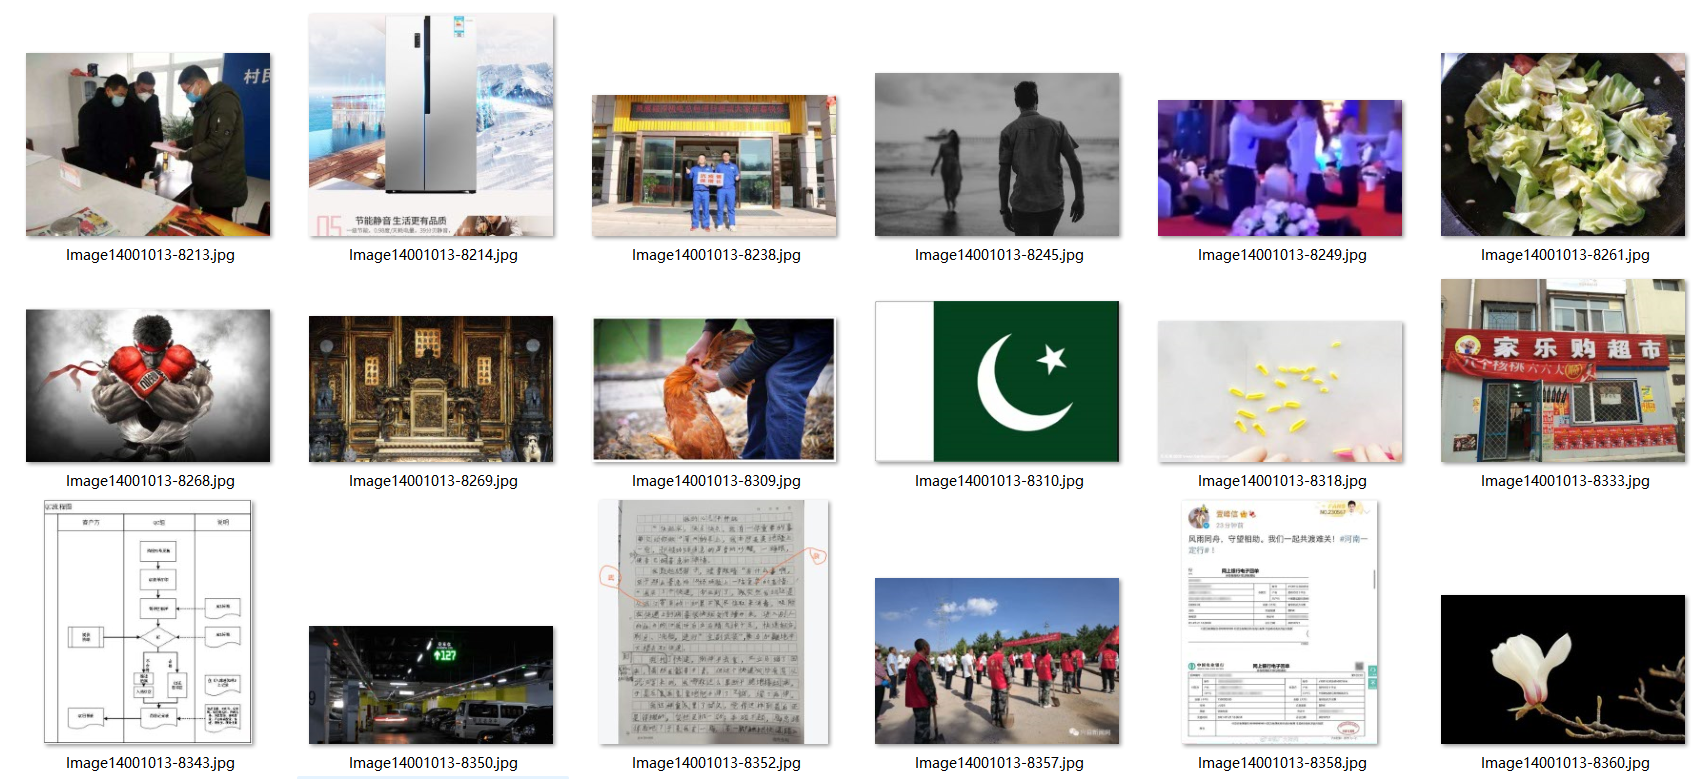
\includegraphics[width=0.95\linewidth]{figures/raw_image}
\caption{原始图像文件概览。}
\label{fig:rawimage}
\end{figure}

按照章节 \ref{modeling} 中提到的方法,我们对每张图像应用随机裁剪、拉伸、双立方下采样等操作,将所有图像的分辨率处理为统一的$224 \times 224$,并对数据进行归一化,以便于后续任务的进行。处理后的结果如图 \ref{fig:cleanimage} 所示。

\begin{figure}[h]
\centering
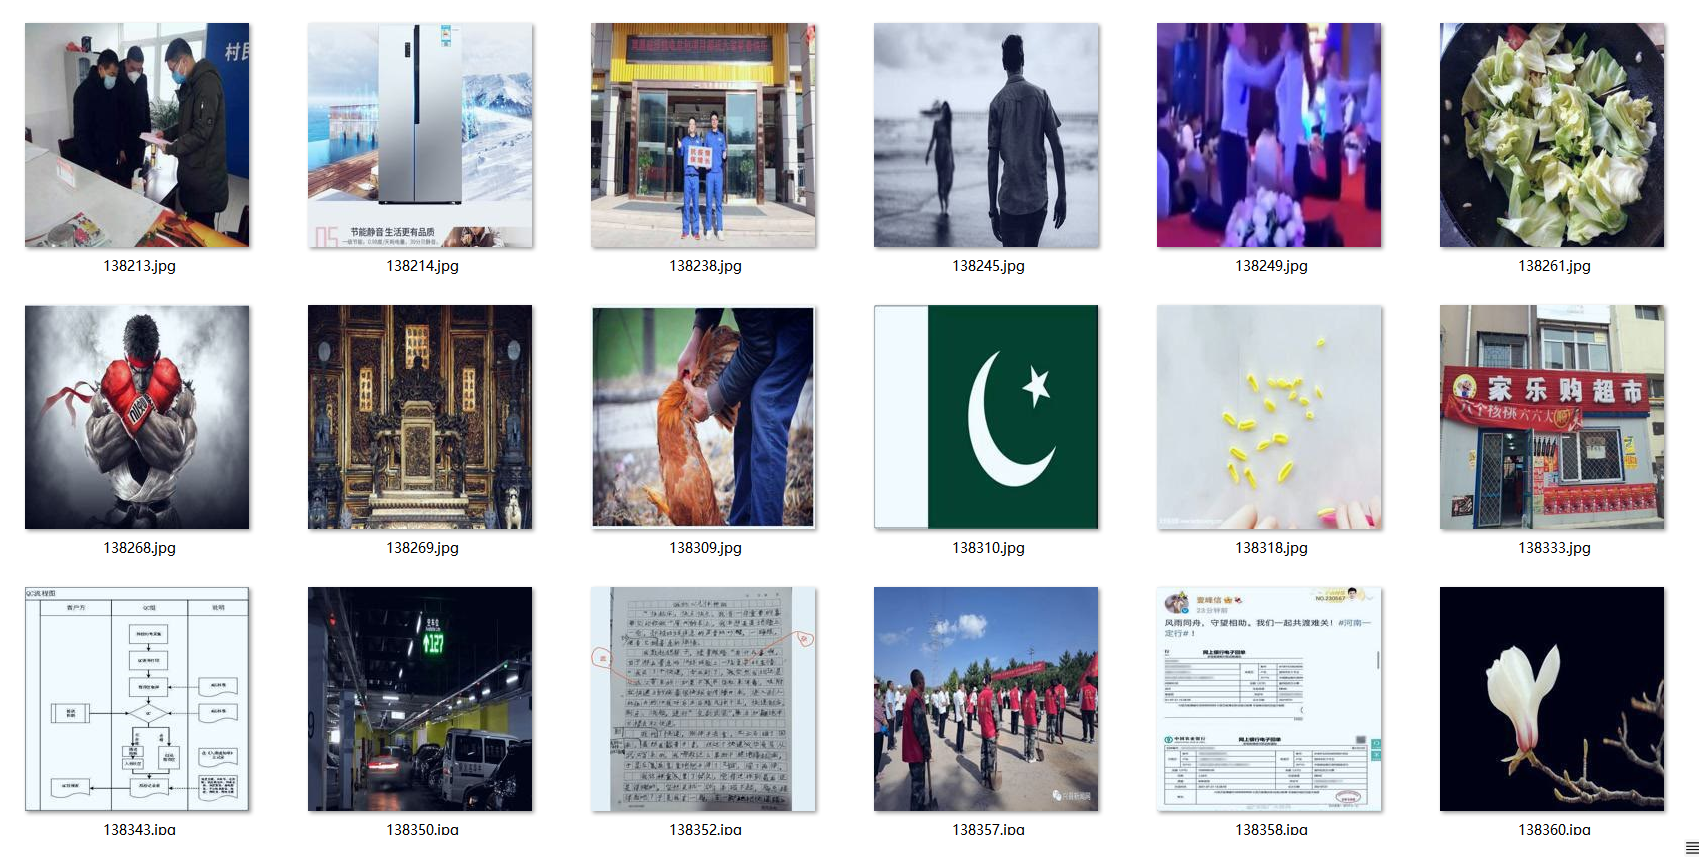
\includegraphics[width=0.95\linewidth]{figures/clean_image}
\caption{处理后的图像文件概览。}
\label{fig:cleanimage}
\end{figure}

\subsubsection{文本异常值处理}

观察给出的文本数据,可以发现这些文本的信息比较杂乱,质量参差不齐,其中包含了很多特殊字符、无用的空白空格和换行、连续出现的标点符号等。

我们使用正则表达式(regex)来识别、替换或删除这些文本中存在的噪声。对文本数据进行清洗有助于确保数据准确、可靠和一致,以用于分析和建模。清洗后的文本样例如图 \ref{fig:cleantext} 所示。

\begin{figure}[h]
\centering
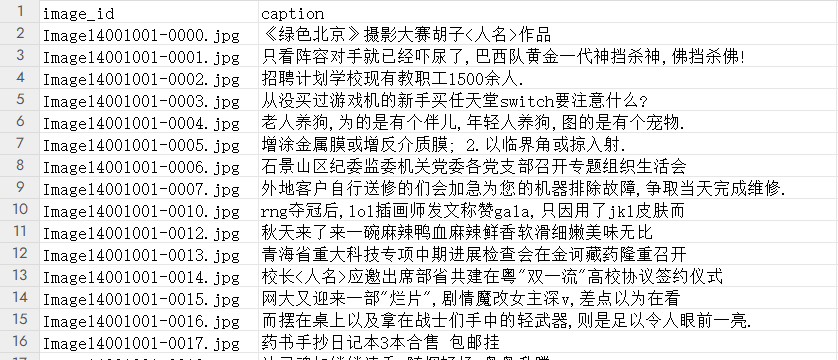
\includegraphics[width=0.95\linewidth]{figures/clean_text}
\caption{处理后的文本示例。}
\label{fig:cleantext}
\end{figure}


\subsection{数据增强}


\subsubsection{图像数据增强}
图像数据增强方法主要分为两类,一种类型的增强涉及数据的空间/几何变换,如裁剪和调整大小、旋转和翻转。 另一种类型的增强涉及外观变换,例如颜色失真(包括颜色下降、亮度、对比度、饱和度、色调)、高斯模糊和 Sobel 过滤。

SimCLR用实验证明了数据增强操作的组合对学习好的表征是至关重要的,而且无监督的对比学习受益于比监督学习更强的数据增强。因此,我们所使用的数据增强操作是这几种方法的组合:
\begin{enumerate}
\item 随机裁剪和调整大小;
\item 随机旋转;
\item 随机翻转;
\item ……。
\end{enumerate}

\subsubsection{文本数据增强}

为了能在不改变原文语义的情况下,生成一定数量的训练语料文本,同时提升模型的泛化性能、干扰波动的能力,我们主要使用以下几种文本数据增强方法:

\begin{enumerate}
\item \textbf{同义词替换:}在这种方法中,我们从句子中随机取出一个词,将其替换为对应的同义词。
\item \textbf{翻译互转:}将文本翻译成另外一种语言,然后再翻译回来。同时,我们也可以翻译成多个语言,从而得到多条回译样本。图 \ref{fig:translate} 演示了该方法的流程。
\end{enumerate}

\begin{figure}[h]
\centering
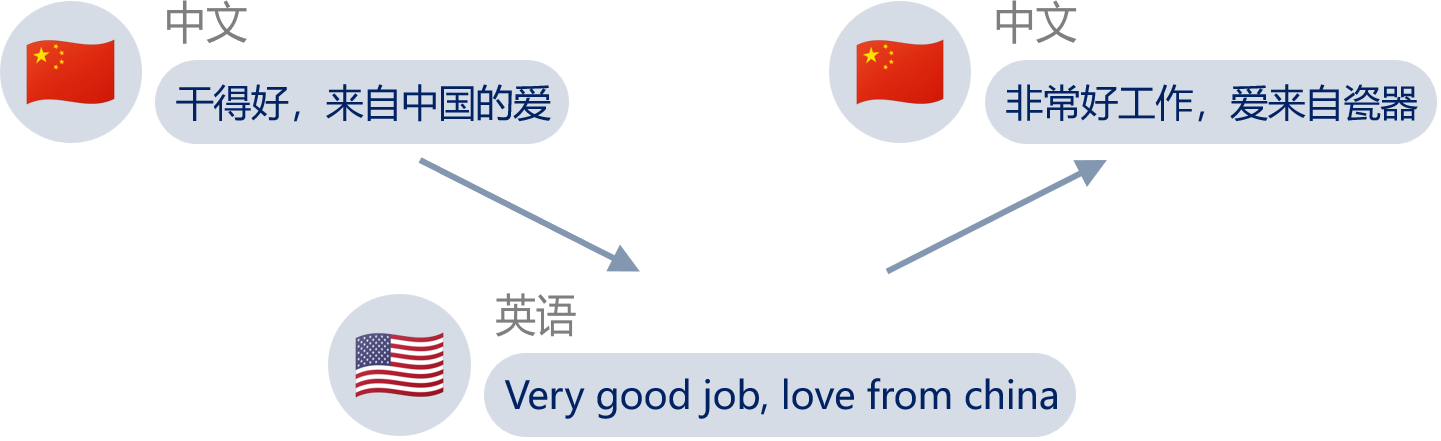
\includegraphics[width=\linewidth]{figures/translate}
\caption{翻译互转示意图。}
\label{fig:translate}
\end{figure}


\subsection{数据集划分}

为了进行训练与测试,我们对“附件1”中的训练集进行了划分,将其中的90\%作为真正的训练集,剩下的10\%作为验证集(这样恰好能使得验证集的大小等于“附件2”和附件“3”中测试集的大小,更加贴近测试环境),用来评估模型的训练效果。根据验证集上的评估指标,我们可以更准确地掌握模型的性能表现,并量化其泛化能力,避免对训练集数据过拟合。具体而言,表 \ref{tbl:DataSplit} 详细说明了数据集的划分情况,以及各个子集的组成。

\begin{table}[h]
\centering
\tabcolsep=1.5em
\renewcommand\arraystretch{1.5}
\caption{\textbf{比赛数据集}划分明细}
\vspace{1em}
\begin{tabular}{c|c|c|c|c}
    \Xhline{2pt}
    数据来源 & \multicolumn{2}{c|}{\textbf{“附件1”}} & \multicolumn{1}{c|}{\textbf{“附件2”}} & 
    \multicolumn{1}{c}{\textbf{“附件3”}}\\
    
%    \Xcline{1-1}{1pt}
    \Xhline{1.5pt}

    数据类型 & \textbf{训练集} & \textbf{验证集} & \textbf{I2T 测试集} & \textbf{T2I 测试集} \\
    \Xhline{0.4pt}
    图像数量 & {45000} & {5000} & {50000(样本)} & {5000(搜索空间)} \\
    \Xhline{0.4pt}
    文本数量 & {45000} & {5000} & {5000(搜索空间)} & {50000(样本)} \\

    \Xhline{2pt}
\end{tabular} \label{tbl:DataSplit}
\end{table}

\subsection{压缩与序列化}

\subsubsection{图像压缩}
为了加快文件读取速度,我们对数据增强后的图像进行JPEG压缩,在保证90\%以上的图像质量前提下,极大地减小了图像的体积。经统计,图像的体积相比未压缩能减少75\%。

\subsubsection{图像序列化}
为保证文件处理效率,我们不是将图片以大量的小文件方式存放,而是将训练/验证/测试图片先经过压缩,再将其字节码序列化为base64格式,分别存放在tsv文件中,每行表示一张图片,包含图片id和图片的base64编码。形式如下:$$\text{“138213	/9j/4AAQSkZJRgABAQAAAQABAAD/2wBDAAgGBgcGBQgHBwcJCQgKDBQ”}$$
这样,便可以避免单独存储大量的图片小文件,而是直接存储一个文本文件。

\subsubsection{文本序列化}
我们将文本信息和图文对的匹配关系保存在JSONL文件中。每行是一个JSON对象,包含文本id、文本内容和匹配的图片id列表。形式如下:
$$\text{“\{"text\_id": 8428, "text": "高级感托特包斜挎", "image\_ids": [10345, 17602]\}”}$$
这样,就可以方便地将文本和图片进行匹配和关联。

\subsubsection{LMDB内存索引}
LMDB 全称为 Lightning Memory-Mapped Database,就是非常快的内存映射型数据库,LMDB使用内存映射文件,可以提供更好的输入/输出性能,对于用于神经网络的大型数据集( 比如 ImageNet ),可以将其存储在 LMDB 中。为了进一步提高模型训练时随机读取数据的效率,我们还需要将tsv和jsonl文件一起序列化,转换为内存索引的LMDB数据库文件,方便训练时的随机读取。

\section{多模态特征融合方法研究}

模态(Modal)是事情经历和发生的方式,我们生活在一个由多种模态(Multimodal)信息构成的世界,包括视觉信息、听觉信息、文本信息、嗅觉信息等等,当研究的问题或者数据集包含多种这样的模态信息时我们称之为多模态问题,研究多模态问题是推动人工智能更好的了解和认知我们周围世界的关键。

每一种信息的来源或者形式,都可以称为一种模态。例如,人有触觉,听觉,视觉,嗅觉;信息的媒介,有语音、视频、文字等;多种多样的传感器,如雷达、红外、加速度计等。以上的每一种都可以称为一种模态。相较于图像、语音、文本等多媒体(Multi-media)数据划分形式,“模态”是一个更为细粒度的概念,同一媒介下可存在不同的模态。 比如我们可以把两种不同的语言当做是两种模态,甚至在两种不同情况下采集到的数据集,亦可认为是两种模态。

在本题目中,我们需要对——图像与文本,这两种模态的数据特征进行融合。

\subsection{算法选择}

多模态检索任务的核心是对多模态数据相似度的度量。在同一维度空间下,人们可以通过欧氏距离、闵式距离等方式来计算两个向量之间的距离。因此,为了比较异构数据的相似度,一个通用的方法是将它们映射到同一个公共表示空间进行相似度的学习。我们首先可以确定任务的解决方案是基于深度学习的多模态特征融合,不同于传统图像处理和传统机器学习算法与简单神经网络的实现,近些年来基于深度学习的多模态模型针对各种复杂应用场景表现性能更好。

在多模态领域,当前的主流模型是基于对比学习的大规模预训练模型。其代表便是CLIP模型。CLIP(Contrastive Language-Image Pre-training)是一个跨模态学习模型\cite{clip},由OpenAI在2021年提出。CLIP模型的核心思想是通过对比学习的方式,将图像和文本映射到同一个嵌入空间中,使得语义上相关的图像和文本在该空间中更接近。

为了更好地理解所使用的改进CLIP模型,下面对相关模型以及使用到的技术进行分别介绍。

\subsection{背景知识}

\subsubsection{对比学习}

对比学习(Contrastive Learning)是一种自监督学习方法\cite{liu2021self},它通过学习数据的相似性和差异性来学习特征的一般表示。其采用的具体思想是将样例和与它语义相似的样本(正样本)及与它语义不相似的样本(负样本)进行对比,通过设计模型结构和对比损失,使语义相近的样本对应的表示在表示空间更接近,语义不相近的例子对应的表示距离更远,以达到类似聚类的效果,如图 \ref{fig:cl1} 所示。

\begin{figure}[h]
\centering
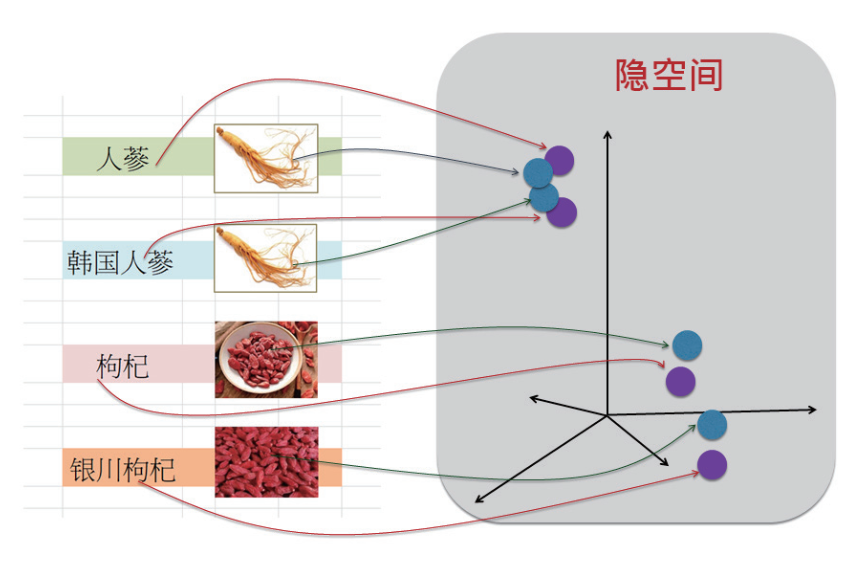
\includegraphics[width=0.75\linewidth]{figures/cl1}
\caption{对比学习示意图。}
\label{fig:cl1}
\end{figure}

\paragraph{对比学习的实施通常包括以下几个方面:}
\begin{enumerate}
\item \textbf{正负样本的定义:}在对比学习中,图像特征和文本特征构成特征矩阵,该矩阵中图文相匹配为正样本,不匹配为负样本,因此特征矩阵的对角线元素均为正样本,其他元素为负样本。
\item \textbf{相似度计算:}使用余弦相似度来表示特征之间的相似度,A、B矩阵的余弦相似度可由公式 \eqref{CosineSim} 描述。
\begin{gather}
\text{Cosine-Similarity}(\mathbf{A}, \mathbf{B})
= {\frac{\mathbf{A} \cdot \mathbf{B}} {\| \mathbf{A} \| \cdot \| \mathbf{B} \|}}
= \frac{\mathbf{A}}{\| \mathbf{A} \|} \cdot \frac{\mathbf{B}}{\| \mathbf{B} \|}
\label{CosineSim}
\end{gather}
\item \textbf{损失函数:}定义一个损失函数来训练模型,使得正样本对的相似度高于负样本对的相似度。典型的损失函数包括三元组损失(Triplet Loss)、对比损失(Contrastive Loss)和交叉熵损失等。公式 \eqref{NCE-Loss} 展示了常用的InfoNCE损失函数的表达式。
\begin{gather}
L_{I}=L_\mathrm{InfoNCE}(z_{i}^{I},z_{i}^{T})=-\frac{1}{N}\Sigma_{i=1}^{N}log\frac{exp(sim(z_{i}^{I},z_{i}^{T})/\tau)}{\Sigma_{j=1}^{N}exp(sim(z_{i}^{I},z_{j}^{T})/\tau)}\label{NCE-Loss}
\end{gather}
\end{enumerate}

\subsubsection{卷积神经网络(CNN)}

卷积神经网络(Convolutional Neural Networks, CNN)这个概念的提出可以追溯到二十世纪80-90年代,但是有那么一段时间这个概念被“雪藏”了,因为当时的硬件和软件技术比较落后,而随着各种深度学习理论相继被提出以及数值计算设备的高速发展,卷积神经网络得到了快速发展。

\begin{figure}[h]
\centering
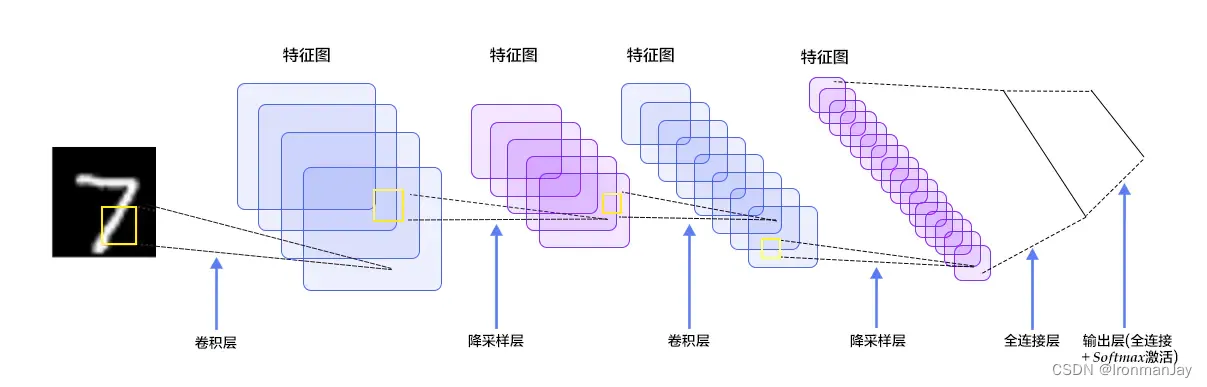
\includegraphics[width=\linewidth]{figures/CNN1}
\caption{卷积神经网络前向过程示意图。}
\label{fig:cnn1}
\end{figure}

卷积神经网络是一种带有卷积结构的深度神经网络,卷积结构可以减少深层网络占用的内存量,其三个关键的操作,其一是局部感受野,其二是权值共享,其三是 pooling 层,有效的减少了网络的参数个数,缓解了模型的过拟合问题。图 \ref{fig:cnn1} 形象地演示了卷积神经网络识别手写数字的推理过程。

\paragraph{卷积神经网络的整体架构可以总结如下:}

\begin{enumerate}
\item 卷积神经网络是一种多层的监督学习神经网络,隐含层的卷积层和池采样层是实现卷积神经网络特征提取功能的核心模块。该网络模型通过采用梯度下降法最小化损失函数对网络中的权重参数逐层反向调节,通过频繁的迭代训练提高网络的精度。
\item 卷积神经网络的低隐层是由卷积层和最大池采样层交替组成,高层是全连接层对应传统多层感知器的隐含层和逻辑回归分类器。
\item 第一个全连接层的输入是由卷积层和子采样层进行特征提取得到的特征图像。
\item 最后一层输出层是一个分类器,可以采用逻辑回归,Softmax 回归甚至是支持向量机对输入图像进行分类。
\end{enumerate}

\begin{figure}[h]
\centering
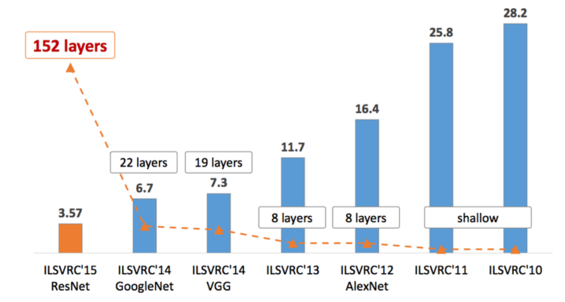
\includegraphics[width=0.85\linewidth]{figures/imagenet}
\caption{ImageNet历届的冠军模型。}
\label{fig:imagenet}
\end{figure}

卷积神经网络再次兴起后,在几年时间内不断地打破ImageNet比赛的最高记录,如图 \ref{fig:imagenet} 所示。具体而言,输入图像统计和滤波器进行卷积之后,提取该局部特征,一旦该局部特征被提取出来之后,它与其他特征的位置关系也随之确定下来了,每个神经元的输入和前一层的局部感受野相连,每个特征提取层都紧跟一个用来求局部平均与二次提取的计算层,也叫特征映射层,网络的每个计算层由多个特征映射平面组成,平面上所有的神经元的权重相等。通常将输入层到隐藏层的映射称为一个特征映射,也就是通过卷积层得到特征提取层,经过 pooling 之后得到特征映射层。

卷积神经网络的核心思想就是局部感受野、是权值共享和pooling层,以此来达到简化网络参数并使得网络具有一定程度的位移、尺度、缩放、非线性形变稳定性。pooling层对图像进行下采样,可以减少数据处理量同时保留有用信息,采样可以混淆特征的具体位置,因为某个特征找出来之后,它的位置已经不重要了,我们只需要这个特征和其他特征的相对位置,可以应对形变和扭曲带来的同类物体的变化。

\subsubsection{Transformer}

Transformer是一种“编码器—解码器”架构,由编码器(encoder)和解码器(decoder)组成,其都是多头自注意力模块的叠加。其中,input sequence分成两部分,分别为源(input)输入序列和目标(output)输出序列。前者输入编码器,后者输入解码器,两个序列均需进行embedding表示并加入位置信息。


\subsubsection{Vision Transformer}

ViT \cite{dosovitskiy2020image} 是Google团队提出的将Transformer \cite{vaswani2017attention} 应用在图像分类的模型,因为其模型“简单”且效果好,可扩展性强,于是成为了Transformer在CV领域应用的里程碑著作,也引爆了后续相关研究。通过在多个基准数据集上的实验对比,表明了ViT可以获得与当时最优卷积神经网络相美的结果。

与传统的卷积神经网络不同,ViT使用自注意力机制代替卷积操作来提取图像特征。由于 Transformer需要的是类似于单词序列的一维输入信号,而图像本身为二维信号,因此在 ViT中,图像被划分成一组固定大小的图像块(patch),每个图像块都被看作是一个序列中的一个元素,然后这些序列元素会被输入到Transformer 模型中,进行特征提取和分类,如图 \ref{fig:vit} 所示。

\begin{figure}[h]
\centering
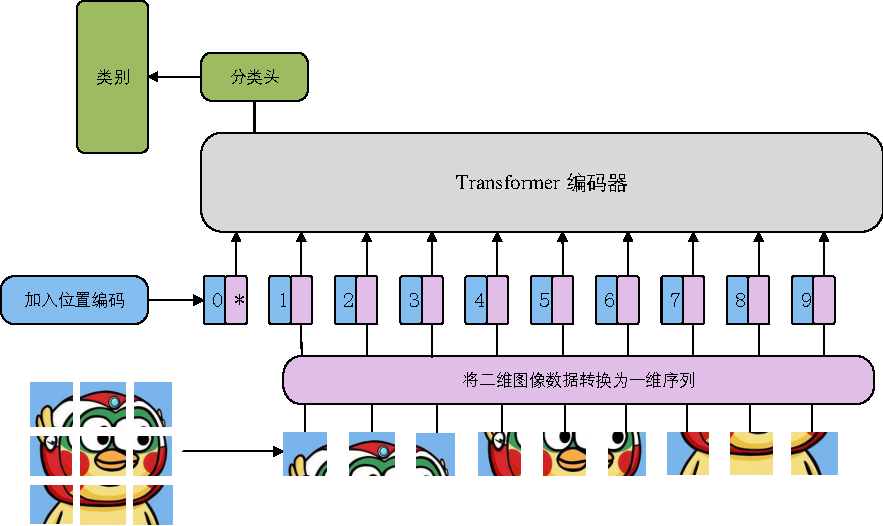
\includegraphics[width=0.9\linewidth]{figures/vit}
\caption{ViT(Vision Transformer)模型结构示意图。}
\label{fig:vit}
\end{figure}

后续 encoder 的操作和原始 Transformer 中完全相同。但是因为对图片分类,因此在输入序列中加入一个特殊的 token,该token 对应的输出即为最后的类别预测。这种序列化的方式可以使得 VT 模型更好地处理全局视觉信息,同时也可以避免卷积神经网络中存在的参数共享限制。ViT 的训练过程可以使用预训练和微调两个阶段。在预训练阶段,VT会使用大量未标记的图像数据来学习视觉特征,而在微调阶段,则会使用少量标记的图像数据来对模型进行微调和分类任务的训练。ViT已经在例如图像分类、目标检测、语义分割等多个视觉任务中取得了很好的表现。 作者根据模型大小(包括“Base”、“Large”和“Huge”)和图像块大小提供了一系列变体,例如 ViT-B/16 表示输入的图像块分辨率是16x16,型号是“Base”其中,Transformer 的序列长度与图像块大小的平方成反比,因此图像块大小越小的模型计算成本越高。


\subsubsection{词向量模型}

词向量模型是将自然语言中的单词转换成固定长度的向量,以便计算机能够更好地理解自然语言的含义。目前,大多数跨模态匹配领域的文本描述都采用单词到向量(Word2vec)和单词表示的全局向量(Glove)两个词向量模型生成单词嵌入。

单词到向量(Word2Vec)是一种通过对输入语料中的单词进行学习,学习其相互关系,从而生成向量表示的模型。其基本思想是通过学习单词在上下文中的分布来捕捉其语义信息。有两种策略可以实现Word2Vec模型:一个是连续词袋模型(Continuous Bag of Words,CBOW),CBOW模型是从周围的单词预测中心单词的概率。

另一个实现单词到向量的策略是采用跳字模型(Skip-gram),这个模型是从中心单词预测周围单词的概率,可以通过学习大规模文本数据的词汇共现关系,将每个单词表示成一个固定长度的向量。单词表示的全局向量(Global Vectors for Word Representation,Glove)旨在通过学习单词的全局共现信息来捕捉词语之间的语义关系。

与Word2Vec中的模型不同,GloVe是在全局语料库中对所有单词对的共现信息进行建模,而不是基于局部的上下文信息来学习词向量。其优点在于能够同时利用全局的词频信息和局部的上下文信息,因此得到的词向量具有较好的语义表示能力。

\subsubsection{BERT}

\begin{figure}[h]
\centering
\includegraphics[width=\linewidth]{figures/bert1}
\caption{BERT(Bidirectional Encoder Representations from Transformers)模型输入示意图。}
\label{fig:bert1}
\end{figure}

\subsection{模型结构}

\begin{figure}[h]
\centering
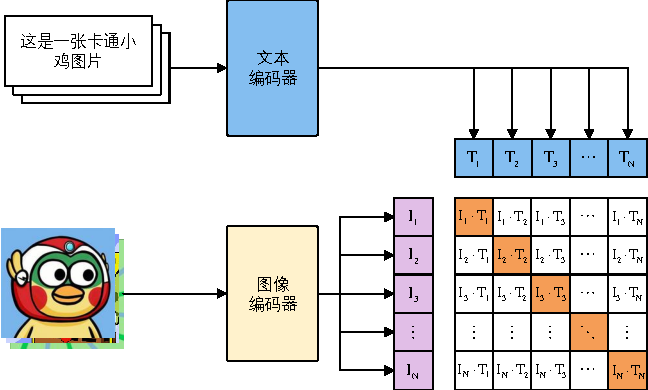
\includegraphics[width=0.95\linewidth]{figures/clip1}
\caption{CLIP(Contrastive Language-Image Pre-training)模型结构示意图。}
\label{fig:clip1}
\end{figure}

CLIP模型的核心思想是通过学习图像和文本之间的匹配关系来提高模型的性能。具体来说,CLIP模型包含两个主要组成部分:一个用于处理图像的CNN模型或ViT模型,和一个用于处理文本的BERT模型。这两个组件都被训练成能够将输入的信息映射到相同的嵌入空间中,并使得相似的图像和文本在嵌入空间中的距离更近。图 \ref{fig:clip1} 演示了CLIP模型的结构。

在实现上,为了兼顾模型精度与效率,我们实现的CLIP模型采用\textbf{ViT-L/14}模型作为图像编码器,以及\textbf{RoBERTa}模型
作为文本编码器。同时,这些编码器均经过充分预训练,显著加快了后续训练的收敛速度。

下面,我们分别介绍使用的预训练图像编码器与文本编码器。

\subsubsection{图像编码器}

ViT \cite{dosovitskiy2020image} 是Google团队提出的将Transformer \cite{vaswani2017attention} 应用在图像分类的模型,因为其模型“简单”且效果好,可扩展性强,于是成为了Transformer在CV领域应用的里程碑著作,也引爆了后续相关研究。

ViT最核心的结论是,当拥有足够多的数据进行预训练的时候,ViT的表现就会超过CNN,突破Transformer缺少归纳偏置的限制,可以在下游任务中获得较好的迁移效果。基于该结论,我们将充分预训练的ViT模型作为CLIP模型的图像编码器,并选择参数量适中的ViT-L/14变种,以平衡精度与计算量的冲突。

具体而言,我们基于HuggingFace平台,获取了在ImageNet数据集中充分预训练的ViT-L/14网络的权重,用来初始化CLIP模型的图像编码器,以获得更佳的迁移学习性能。


\subsubsection{文本编码器}

RoBERTa \cite{roberta} 是在论文\emph{RoBERTa: A Robustly Optimized BERT Pretraining Approach}中被提出的。此方法属于BERT的强化版本,也是BERT模型更为精细的调优版本。RoBERTa主要在三方面对之前提出的BERT做了该进,其一是模型的具体细节层面,改进了优化函数;其二是训练策略层面,改用了动态掩码的方式训练模型,证明了NSP(Next Sentence Prediction)训练策略的不足,采用了更大的Batch Size;其三是数据层面,一方面使用了更大的数据集,另一方面是使用字节级别的BPE(Bytes-level BEP )来处理文本数据。

RoBERTa在训练方面与原始BERT模型保持一致,使用类似“完形填空”的代理任务,让模型学习填补缺失词。输入句子中部分词被随机遮掩,替换为“[PAD]”,并在最前方添加一个特殊词汇“[CLS]”。对于缺失值填补任务,要求“[PAD]”的输出能还原原始词汇;对于分类任务,使用“[CLS]”的输出作为分类器的特征。

与图像编码器类似,我们使用基于中文数据预训练的RoBERTa模型 \cite{cn-roberta} 作为CLIP的文本编码器。该策略极大地提高了CLIP模型预训练与微调的效率,使得我们能在有限的训练回合中,获得更大的精度收益。


\subsection{训练目标}

CLIP使用图像文本对作为训练标签。这里举例一个包含$N$个图像文本对的训练Batch,对提取的文本特征和图像特征进行训练的过程:

\begin{enumerate}
\item 输入图像 $\rightarrow$ 图像编码器 $\rightarrow$ 图像特征向量;输入文字 $\rightarrow$ 文字编码器 $\rightarrow$ 文字特征向量;并进行线性投射,得到相同维度;
\item 将$N$个图像特征和$N$个文本特征两两组合,形成一个形状为$N \times N$的矩阵$s$;
CLIP模型会预测计算出这$N^2$个图像文本对的相似度(即余弦相似度);
\item 对角线上的N个元素因为图像-标签对应正确被作为训练的正样本,剩下的$N(N-1)$个元素作为负样本;
\item CLIP的训练目标是基于对比损失,最大化$N$个正样本的相似度,同时最小化$N(N-1)$个负样本的相似度。
\end{enumerate}

具体而言,对于任意一个图像文本对,CLIP的对比损失如公式 \eqref{loss_one} 所示。最后考虑所有可能存在的图像文本对,需要最小化的目标函数如公式 \eqref{loss_all} 所示。其中,$s_{i,j}$表示相似度矩阵第$i$行的第$j$列的元素,其数值含义为第$i$幅图像与第$j$段文本的相似度,由公式 \eqref{CosineSim} 计算。
\begin{gather}
l(i,j)=-\log\frac{\exp(s_{i,j})}{\sum_{k=1}^{N} \mathbf{1}_{\left[k \ne i\right]} \exp(s_{i,k})}\label{loss_one}\\
\mathcal{L}=\frac{1}{2N}\sum_{k=1}^N[l(k-1,k)+l(k,k-1)]\label{loss_all}
\end{gather}


\subsection{模型推理} \label{infer}

基于上述损失函数,我们在大规模数据集上对CLIP模型训练后,得到的权重可以用于推理。这里,我们以问题一的I2T任务为例,演示CLIP进行图像检索文本推理的过程。

\subsubsection{数据预处理}

设我们进行I2T任务的目标图像为$Image_1$,潜在文本集合为$\{Text_i \mid 1 \le i \le N\}$。模型首先对目标图像进行预处理,通过裁剪、缩放和插值操作,得到结构化的图像 $X \in \mathbb{R}^{1 \times H \times W \times C}$。对于原始类别标签,我们将其拼接至模板“这是一张\{XX\}图像”中,使其更符合中文语法习惯,如图 \ref{fig:clip2} 所示。接下来,对拼接后的文本进行处理,将其分词后映射至词汇表,通过填充与截断操作控制序列长度,并转换为训练得到的词向量矩阵,得到结构化的文本$Y \in \mathbb{R}^{N \times L \times D_\mathrm{emb}}$。

\subsubsection{图像文本编码}

\begin{figure}[h]
\centering
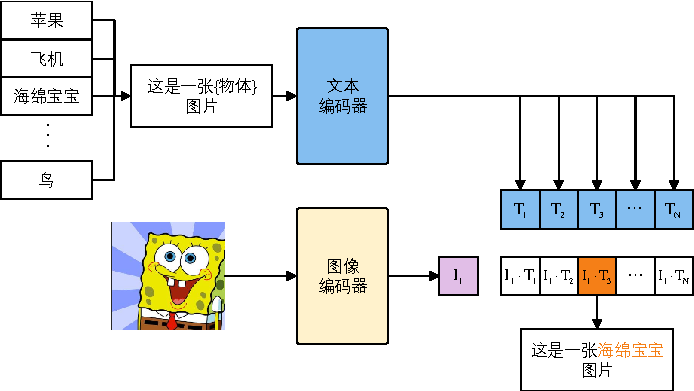
\includegraphics[width=0.9\linewidth]{figures/clip2}
\caption{CLIP模型推理——图像检索文本}
\label{fig:clip2}
\end{figure}

对于结构化的图像与文本数据,使用CLIP的图像编码器与文本编码器,将其映射至同维度的编码向量。为了计算方便,我们对所有编码向量进行归一化,得到归一化图像编码$I \in \mathbb{R}^{1 \times D_\mathrm{model}}$以及归一化文本编码$T \in \mathbb{R}^{N \times D_\mathrm{model}}$。对于任意图像$Image_i$和文本$Text_j$,其归一化编码的计算过程分别如公式 \eqref{NormImage} 和公式 \eqref{NormText} 所示。通过进行归一化,我们可以使用向量的点乘操作来替代此前的余弦相似度计算。
\begin{gather}
I_i = \frac{r_i}{\|r_i\|}\label{NormImage}\quad \text{其中,}
r_i = \mathrm{ImageEncoder}\left(Image_i\right)\\
\vspace{1em}
T_j = \frac{h_j}{\|h_j\|}\label{NormText}\quad \text{其中,}
h_j = \mathrm{TextEncoder}\left(Text_j\right)
\end{gather}

\subsubsection{相似度计算}

接下来,对目标图像编码$I_1$与所有文本编码$T$进行点乘,得到目标图像与各段文本的相似度数组$\mathrm{Sims} = \{I_1 \cdot T_i \mid 1 \le i \le N\}$。最后,取相似度数组Sims的最大值,与之对应的文本即为最佳匹配文本。类似的,若取最大的$K$个值,则可得到最佳的$K$段匹配文本。图 \ref{fig:clip2} 演示了CLIP模型进行图像检索文本推理的完整流程。

\subsection{改进策略}

\subsubsection{梯度累积(Gradient Accumulation)}

在深度学习训练的时候,数据的batch size大小受到GPU内存限制,batch size大小会影响模型最终的准确性和训练过程的性能。在GPU内存不变的情况下,模型越来越大,那么这就意味着数据的batch size只能缩小。然而,有研究表示主流的对比学习模型通常batch size越大,训练过程越平稳,最终的性能表现也越好。

通常,当一块GPU的内存不足时,可以采用多GPU进行分布式训练。将一个大的Batch均摊到多块GPU上,计算完梯度后再汇总,进行梯度下降,如图 \ref{fig:grad} 所示。然而,分布式训练会带来额外的通讯与同步开销,且成本高昂。

\begin{figure}[h]
\centering
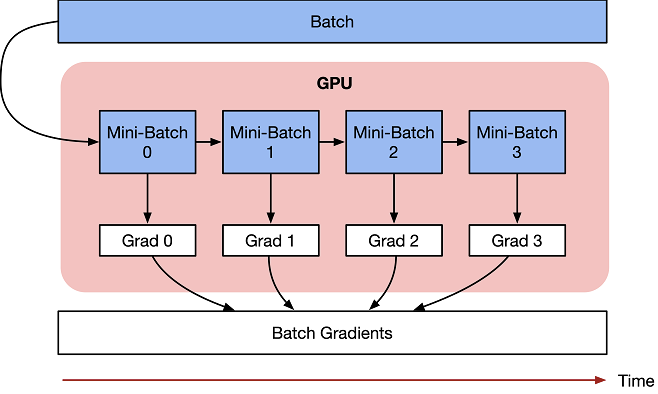
\includegraphics[width=0.9\linewidth]{figures/grad}
\caption{分布式训练示意图。}
\label{fig:grad}
\end{figure}


这个时候,梯度累积(Gradient Accumulation)可以作为一种简单的解决方案来解决这个问题。梯度累积是一种不需要额外硬件资源就可以增加批量样本数量(Batch Size)的训练技巧。这是一个通过时间换空间的优化措施,它将多个Batch训练数据的梯度进行累积,在达到指定累积次数后,使用累积梯度统一更新一次模型参数,以达到一个较大Batch Size的模型训练效果。累积梯度等于多个Batch训练数据的梯度的平均值。

所谓梯度累积过程,其实很简单,我们梯度下降所用的梯度,实际上是多个样本算出来的梯度的平均值,以batch\_size=1024为例,你可以一次性算出1024个样本的梯度然后平均,我也可以每次算64个样本的平均梯度,然后缓存累加起来,算够了16次之后,然后把总梯度除以16,然后才执行参数更新。当然,必须累积到了16次之后,用16次的平均梯度才去更新参数,不能每算64个就去更新一次,不然就是batch\_size=64了。该过程可以由以下列表描述:

\begin{enumerate}
\item 正向传播,出入数据,得到预测结果;
\item 根据预测结果与label,计算损失值;
\item 利用损失进行反向传播,计算参数梯度;
\item 重复上面步骤,不清空梯度,将梯度累加;
\item 梯度累加达到固定次数之后,更新参数,然后将梯度清零.
\end{enumerate}

总结来讲,梯度累积就是每计算一个batch的梯度,不进行清零,而是做梯度的累加,当累加到一定的次数(accumulation\_steps)之后,再更新网络参数,然后将梯度清零。通过这种参数延迟更新的手段,可以实现与采用大batch size相近的效果。在平时的实验过程中,我一般会采用梯度累加技术,大多数情况下,采用梯度累加训练的模型效果,要比采用小batch size训练的模型效果要好很多。

\subsubsection{掩码特征学习}

我们借鉴了FLIP模型的图像掩码策略,对CLIP模型进行改进。我们首先将图像划分为不重叠的 patch,随机屏蔽掉大部分(例如 50\% 或 75\%)的 patch,图像编码器仅应用于可见 patch。

与原始的CLIP模型相比,改进后的模型在同样的训练时间内可以学习更多的图像-文本对,并且ImageEncoder的显存使用也下降(mask掉50\%,显存消耗就下降50\%),这样在一定的硬件资源下就可以实现更大的batch size,而对比学习往往需要较大的batch size。同时,由于图像往往具有较强的冗余性,即使mask大部分图像,特征网络的学习性能并不会变差,反而由于更大的batch size而可以获得更好的性能。

\begin{figure}[h]
\centering
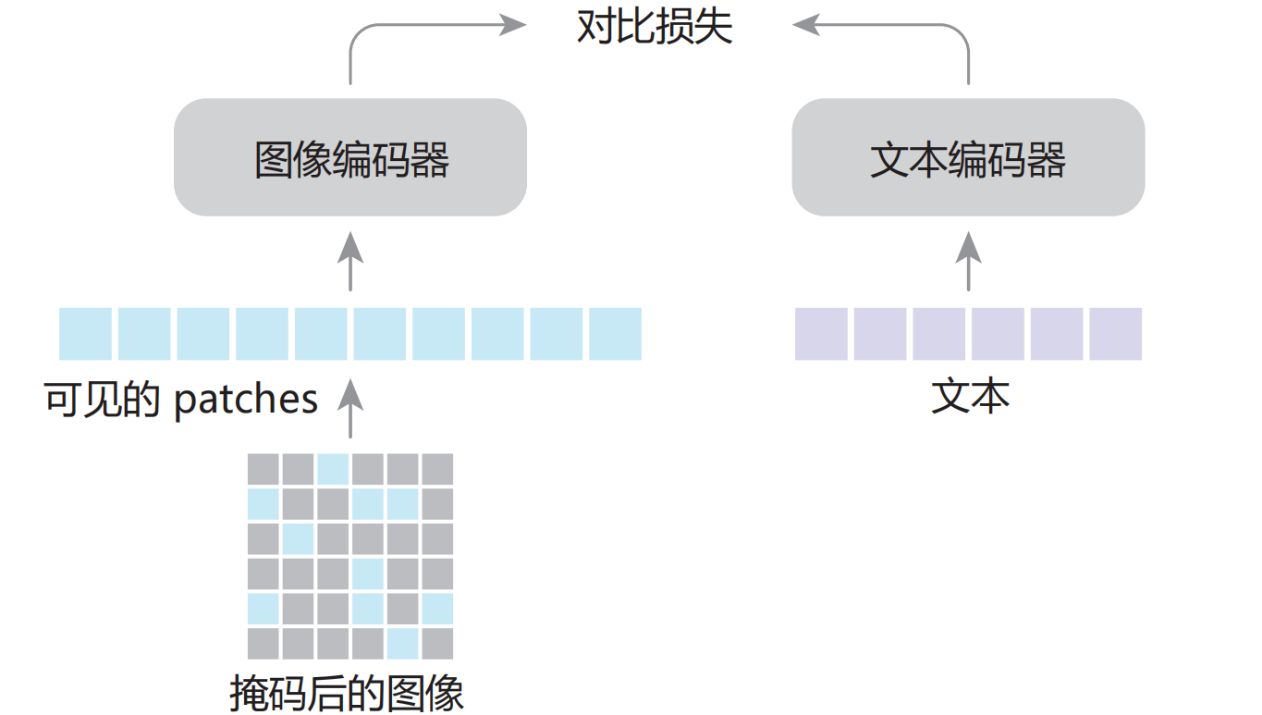
\includegraphics[width=0.95\linewidth]{figures/mask}
\caption{掩码特征学习示意图。}
\label{fig:mask}
\end{figure}

综上,FLIP使用类似MAE模型的掩码输入策略,减少了编码序列的长度,极大地节省了显存的消耗量,使得我们可以使用更大的batch size进行训练,以获得更佳的泛化性能。


\subsubsection{FlashAttention}

在标准注意力实现中,注意力的性能主要受限于内存带宽,是内存受限的。频繁地从HBM中读写 $\mathbb{R}^{N \times N}$ 的矩阵是影响性能的主要瓶颈。稀疏近似和低秩近似等近似注意力方法虽然减少了计算量FLOPs,但对于内存受限的操作,运行时间的瓶颈是从HBM中读写数据的耗时,减少计算量并不能有效地减少运行时间(wall-clock time)。针对内存受限的标准注意力,Flash Attention是IO感知的,目标是避免频繁地从HBM中读写数据。图 \ref{fig:flash} 以一个金字塔的形式,形象地说明了GPU中各存储器的IO效率差异。

\begin{figure}[h]
\centering
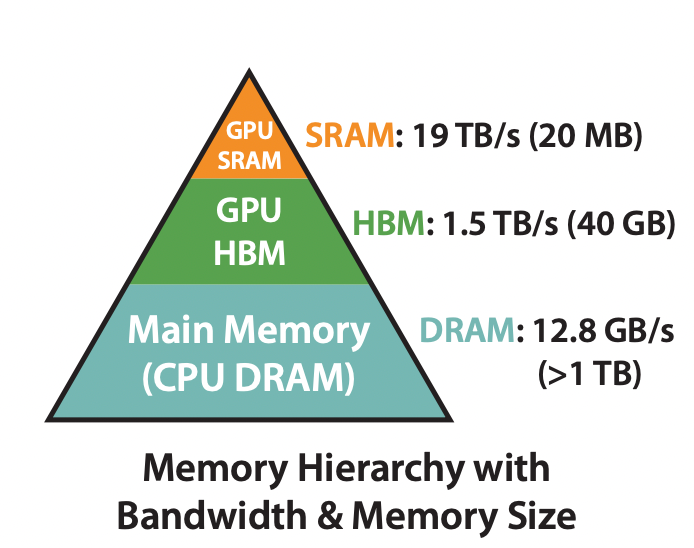
\includegraphics[width=0.5\linewidth]{figures/flash}
\caption{GPU中的IO速度金字塔。}
\label{fig:flash}
\end{figure}


从GPU显存效率分级来看,SRAM的读写速度比HBM高一个数量级,但内存大小要小很多。通过kernel融合的方式,将多个操作融合为一个操作,利用高速的SRAM进行计算,可以减少读写HBM的次数,从而有效减少内存受限操作的运行时间。但SRAM的内存大小有限,不可能一次性计算完整的注意力,因此必须进行分块计算,使得分块计算需要的内存不超过SRAM的大小。

Flash Attention的作者将多头注意力的计算抽象为以下操作:
\begin{gather}
S=\tau QK^{\top}\in\mathbb{R}^{N\times N} \\
S^\text{masked }=MASK(S)\in\mathbb{R}^{N\times N} \\
P=\mathrm{softmax}\left(S^{\mathrm{masked}}\right)\in\mathbb{R}^{N\times N} \\
P^{\mathrm{dropped}}=\mathrm{dropout} (P,p_{\mathrm{drop}} )\in\mathbb{R}^{N\times N} \\
O=P^{\mathrm{dropped}}V\in\mathbb{R}^{N\times d} 
\end{gather}

为了提高运算效率,在Flash Attention算法中,并没有将$\mathbf{S}\text{、}\mathbf{P}$写入HBM中去,而是通过分块写入到HBM中去,存储前向传递的 softmax 归一化因子,在后向传播中快速重新计算片上注意力,这比从HBM中读取中间注意力矩阵的标准方法更快。即使由于重新计算导致 FLOPS 增加,但其运行速度更快并且使用更少的内存(序列长度线性),主要是因为大大减少了 HBM 访问量。

简而言之,Flash Attention实现了不使用中间注意力矩阵,通过存储归一化因子来减少HBM内存的消耗,同时减少了HBM访问量,使得Attention计算过程中在IO方面的开销大大减少,从而提高了前向运算的速度,并降低了显存的开销。

\section{实验与结果分析}

\subsection{模型预训练}

\subsubsection{数据集构建}
在预训练阶段,我们首先根据MUGE Retrieval、Flickr30K-CN、COCO-CN这三个中文检索方向常用数据集构建了约800万样本的数据集。为了确保数据集的质量,我们对数据集进行了彻底的清洗,移除了重复项、低分辨率图像以及包含错误或不完整文本的样本。此外,我们还执行了数据增强,图像包括随机裁剪、翻转、旋转,文本包括同义词替换、翻译互转等操作,以增加数据的多样性并提高模型对不同图像变换的鲁棒性。在数据清洗过程中,需要保持数据的多样性和代表性,确保模型能够学习到丰富的视觉和语言特征,同时使数据分布尽量平衡,防止模型模型出现偏向性。
数据增强策略的实施,旨在模拟真实世界条件下图像可能出现的各种情况,以增强模型的泛化性。通过这种方式,能够提升模型对于图像几何变换的适应能力。


\subsubsection{模型预训练}



\subsubsection{“零样本”测试}

在仅基于公共数据集预训练,\textbf{不使用任何比赛数据集相关信息}的情况下,对模型进行性能评估,称为“零样本”测试。具体而言,我们按照章节 \ref{infer} 中描述的方法,使用基于公共数据集预训练的模型,在比赛数据集的\textbf{I2T测试集}和\textbf{T2I测试集}上进行测试。

为了进行更全面的性能评估,我们除了计算题目所要求的R@5指标,还分别计算了R@1、R@10指标,以及各个指标的均值MR。

\paragraph{图像检索文本}

按照章节 \ref{infer} 中描述的方法,我们使用基于公共数据集预训练的模型,在比赛数据集的I2T测试集上进行测试。

\begin{table}[h]
\centering
\tabcolsep=1.5em
\renewcommand\arraystretch{1.5}
\caption{\textbf{“零样本”}测试结果——\textbf{图像检索文本}}
\vspace{1em}
\begin{tabular}{c|cccc}
    \Xhline{2pt}

    回合 $\backslash$ 评估指标 & \textbf{R@1} & \textbf{R@5} & \textbf{R@10} & \textbf{MR} \\
    
    \Xcline{1-1}{0.4pt}
    \Xhline{1.5pt}

    1 epoch & {0.3814} & {0.5800} & {0.6562} & {0.5392} \\
    \Xhline{0.4pt}
    2 epochs & {0.3814} & {0.5800} & {0.6562} & {0.5392} \\
    \Xhline{0.4pt}
    3 epochs & {0.3814} & {0.5800} & {0.6562} & {0.5392} \\
    \Xhline{0.4pt}
    4 epochs & {0.3814} & {0.5800} & {0.6562} & {0.5392} \\
    \Xhline{0.4pt}
    5 epochs & {0.5156} & {0.7094} & {0.7712} & {0.6654} \\
    
    \Xhline{2pt}
\end{tabular} \label{tbl:Zero1}
\end{table}

\paragraph{文本检索图像}

\begin{table}[h]
\centering
\tabcolsep=1.5em
\renewcommand\arraystretch{1.5}
\caption{\textbf{“零样本”}测试结果——\textbf{图像检索文本}}
\vspace{1em}
\begin{tabular}{c|cccc}
    \Xhline{2pt}

    回合 $\backslash$ 评估指标 & \textbf{R@1} & \textbf{R@5} & \textbf{R@10} & \textbf{MR} \\
    
    \Xcline{1-1}{0.4pt}
    \Xhline{1.5pt}

    1 epoch & {0.3814} & {0.5800} & {0.6562} & {0.5392} \\
    \Xhline{0.4pt}
    2 epochs & {0.3814} & {0.5800} & {0.6562} & {0.5392} \\
    \Xhline{0.4pt}
    3 epochs & {0.3814} & {0.5800} & {0.6562} & {0.5392} \\
    \Xhline{0.4pt}
    4 epochs & {0.3814} & {0.5800} & {0.6562} & {0.5392} \\
    \Xhline{0.4pt}
    5 epochs & {0.5156} & {0.7094} & {0.7712} & {0.6654} \\
    
    \Xhline{2pt}
\end{tabular} \label{tbl:Zero2}
\end{table}

\subsection{模型微调}

\subsubsection{数据集构建}
我们使用比赛附件1中所给的数据构建微调模型所使用的数据集,对数据集进行增强,如对图像进行随机裁剪、翻转、旋转,对文本进行同义词替换、翻译互转,人为地增加了数据的多样性,有助于模型学习到更加鲁棒的特征,从而在面对未见过的样本时能够做出准确的预测。
在数据集准备好之后,我们将其划分为训练集、验证集和测试集,以便在训练过程中监控模型的性能,并最终评估其泛化能力。同时我们采用交叉验证的方法,以确保模型在不同的数据子集上都能保持一致的性能。
\subsubsection{模型微调}

\subsubsection{微调结果测试}




\subsection{结果分析}

\subsubsection{预训练结果}

\subsubsection{微调结果}

\subsubsection{有效性验证}

\subsection{模型总结}


\cite{*}

\newpage

\addcontentsline{toc}{section}{参考文献}

\bibliographystyle{ieeetr}
\bibliography{./bib/MyRefs}


\end{document}
